\begin{figure}
\center

Ground Truth: $p = 0$


\begin{comment}
python3 CounterfactualModel_VIZ.py 0 0 10.0 180 FOURIER_101 FOURIER_201 2345
python3 CounterfactualModel_VIZ.py 0 0 10.0 180 FOURIER_102 FOURIER_202 2345
python3 CounterfactualModel_VIZ.py 0 0 10.0 180 FOURIER_103 FOURIER_203 2345


python3 RunSynthetic_FreePrior_ZeroTrig_OnSim_VIZ.py 0 0 10.0 180 SimulateSynthetic_Parameterized_OtherNoiseLevels_Grid_VarySize_ZeroTrig.py_180_0_2345_N10000_FOURIER_101_FOURIER_201.txt
python3 RunSynthetic_FreePrior_ZeroTrig_OnSim_VIZ.py 0 0 10.0 180 SimulateSynthetic_Parameterized_OtherNoiseLevels_Grid_VarySize_ZeroTrig.py_180_0_2345_N10000_FOURIER_102_FOURIER_202.txt
python3 RunSynthetic_FreePrior_ZeroTrig_OnSim_VIZ.py 0 0 10.0 180 SimulateSynthetic_Parameterized_OtherNoiseLevels_Grid_VarySize_ZeroTrig.py_180_0_2345_N10000_FOURIER_103_FOURIER_203.txt

python3 evaluateCrossValidationResults_Synthetic_Gardelle.py SimulateSynthetic_Parameterized_OtherNoiseLevels_Grid_VarySize_ZeroTrig.py_180_0_2345_N10000_FOURIER_101_FOURIER_201.txt
python3 evaluateCrossValidationResults_Synthetic_Gardelle.py SimulateSynthetic_Parameterized_OtherNoiseLevels_Grid_VarySize_ZeroTrig.py_180_0_2345_N10000_FOURIER_102_FOURIER_202.txt
python3 evaluateCrossValidationResults_Synthetic_Gardelle.py SimulateSynthetic_Parameterized_OtherNoiseLevels_Grid_VarySize_ZeroTrig.py_180_0_2345_N10000_FOURIER_103_FOURIER_203.txt
\end{comment}



Example 1

\begin{minipage}[c]{0.8\linewidth}
\sideimage{Fitted}{figures/CounterfactualModel_VIZ.py_2345_FOURIER_101_FOURIER_201_0_0_10.0_180.pdf}

\sideimage{Fitted}{figures/RunSynthetic_FreePrior_ZeroTrig_OnSim_VIZ.py_SimulateSynthetic_Parameterized_OtherNoiseLevels_Grid_VarySize_ZeroTrig.py_180_0_2345_N10000_FOURIER_101_FOURIER_201.txt_0_0_10.0_180.pdf}
\end{minipage}
\begin{minipage}[c]{0.19\linewidth}
\centering

\ \ \ \ \ \ Negative

\ \ \ \ \ \ Log-Likelihood

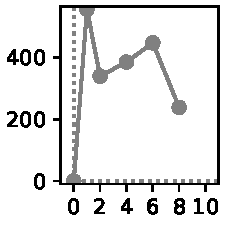
\includegraphics[width=0.98\textwidth]{figures/evaluateCrossValidationResults_Synthetic_Gardelle.py_SimulateSynthetic_Parameterized_OtherNoiseLevels_Grid_VarySize_ZeroTrig.py_180_0_2345_N10000_FOURIER_101_FOURIER_201.txt_RelativeLF.pdf}
\end{minipage}

\ 

Example 2

\begin{minipage}[c]{0.8\linewidth}
\sideimage{Fitted}{figures/CounterfactualModel_VIZ.py_2345_FOURIER_102_FOURIER_202_0_0_10.0_180.pdf}

\sideimage{Fitted}{figures/RunSynthetic_FreePrior_ZeroTrig_OnSim_VIZ.py_SimulateSynthetic_Parameterized_OtherNoiseLevels_Grid_VarySize_ZeroTrig.py_180_0_2345_N10000_FOURIER_102_FOURIER_202.txt_0_0_10.0_180.pdf}
\end{minipage}
\begin{minipage}[c]{0.19\linewidth}
\centering

\ \ \ \ \ \ Negative

\ \ \ \ \ \ Log-Likelihood

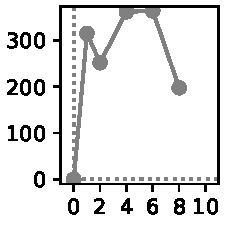
\includegraphics[width=0.98\textwidth]{figures/evaluateCrossValidationResults_Synthetic_Gardelle.py_SimulateSynthetic_Parameterized_OtherNoiseLevels_Grid_VarySize_ZeroTrig.py_180_0_2345_N10000_FOURIER_102_FOURIER_202.txt_RelativeLF.pdf}
\end{minipage}

\ 

Example 3

\begin{minipage}[c]{0.8\linewidth}
\sideimage{Fitted}{figures/CounterfactualModel_VIZ.py_2345_FOURIER_103_FOURIER_203_0_0_10.0_180.pdf}

\sideimage{Fitted}{figures/RunSynthetic_FreePrior_ZeroTrig_OnSim_VIZ.py_SimulateSynthetic_Parameterized_OtherNoiseLevels_Grid_VarySize_ZeroTrig.py_180_0_2345_N10000_FOURIER_103_FOURIER_203.txt_0_0_10.0_180.pdf}
\end{minipage}
\begin{minipage}[c]{0.19\linewidth}
\centering

\ \ \ \ \ \ Negative

\ \ \ \ \ \ Log-Likelihood


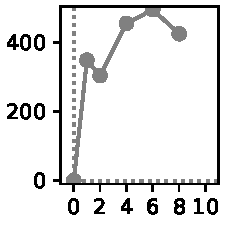
\includegraphics[width=0.98\textwidth]{figures/evaluateCrossValidationResults_Synthetic_Gardelle.py_SimulateSynthetic_Parameterized_OtherNoiseLevels_Grid_VarySize_ZeroTrig.py_180_0_2345_N10000_FOURIER_103_FOURIER_203.txt_RelativeLF.pdf}
\end{minipage}


\caption{Supplement to Figure 4: Randomly constructed models.
We simulate three models at the ground truth loss function exponent indicated.
The loss function is clearly identified by model fit, and, when fitting at this loss, prior and encoding are recovered.
See Section~\ref{sec:att-rep} for discussion of Attraction and Repulsion components.
}
\label{fig:fourier-0}
\end{figure}


